In this chapter I will show the behaviour of task-affinity on different architectures. First of all, using \textit{trace}, we will check if expected 
scheduling is performed, after which we will analyze how optimization proposed influences performance and L1 and LLC miss rates of the application. 

In Fig. \ref{fig:ideal_scheduling} they are represented the ideal scheduling that the developed patch and vanilla should perform. 
I have said "ideal" because, as described in \cite{lcs}, it is impossible to perform these scheduling, because scheduling latencies are not equal for each 
core.

\begin{figure}[htbp]
\centering
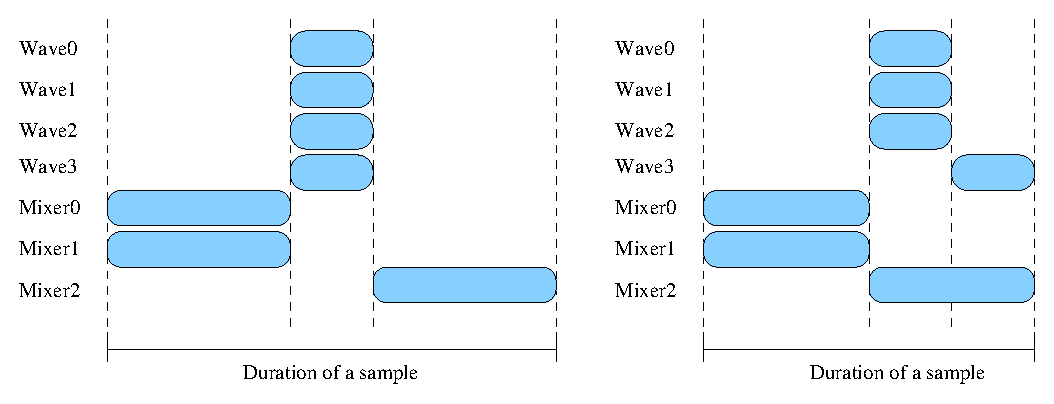
\includegraphics[width=\widefigure]{images/schedule_van_taskaff.eps}
\caption{\figurecaption{Ideal Scheduling performed by vanilla (left figure) and task-affinity (right figure).}}
\label{fig:ideal_scheduling}
\end{figure}

For simplicity, in the pictures we have assumed that all \textit{mixers} and all \textit{waves} have the same duration and a \textit{mixer} takes twice the 
time it takes for a \textit{wave}. In the real benchmark, durations of the \textit{waves} are slightly different, durations of the \textit{mixer0} and 
\textit{mixer1} are slightly different, \textit{mixer2} takes more time than \textit{mixer0} or \textit{mixer1}.

Considering time normalized to the duration of one sample, it is possible express durations of different tasks in relative terms.
Using relative durations, it is possible to estimate the improvement given by task-affinity using the \textit{amdhal's law} \cite{lcs}:

\begin{equation}
       Speedup = \left(\frac{P_{1}}{S_{1}} + \frac{P_{2}}{S_{2}} + ... \frac{P_{n}}{S_{n}} \right)^{-1} 
\label{eq:amdhal}
\end{equation}

Where $P_{i}$ is the i-th parallelized portion of the program and $S_{i}$ is the correspondent parallelization factor. Furthermore the following constraint 
must be respected:

\begin{equation}
       \sum_{i=1}^N P_{i} = 1
\label{eq:contr_amdhal}
\end{equation}
\newpage

%%%%%%%%%%%%%%%%%%%%%%%%%%%%%%%%%%%%%%%%%%%%%%%%%%%%%%%%%%%%%%%%%%%%%%%%%%%%%
\section{Comparing to vanilla}

In this section, we analyze the behaviour of optimized task-affinity on different architectures. First of all, we desire to know if scheduling performed by 
task-affinity on different architectures approximates the ideal scheduling showed in Fig. \ref{fig:ideal_scheduling} and if, as we expected, this 
scheduling improves throughput of the application. The improvement of throughput was measured using the Amdhal's Law \ref{eq:amdhal}. We have measured the 
theoretical speedup given by task-affinity, executing the following experiment:

\begin{enumerate}
\item We have executed benchmark with only one cpu online for each buffer dimension. In this way, benchmark is executed in a serialized way.
\item We have recorded average execution time of each thread of the benchmark, and the average execution time of a sample.
\item We have divided the serial execution of benchmark in different portions according to parallelization. For vanilla, we have three portions: $P_{0}$ 
that includes the sum of execution time of \textit{mixer0} and \textit{mixer1}, $P_{1}$ that includes the sum of execution time of \textit{waves}, $P_{2}$ 
that includes the execution time of \textit{mixer2}. To determine which is the parallelization of each portion, we have made some approximations, such as: 
all \textit{waves} have the same duration, \textit{mixer0} and \textit{mixer1} have the same duration. Thanks to these approximations, we can approximate 
the scheduling performed by vanilla with the ideal scheduling. In this way, $P_{0}$ have a parallelization factor of $S_{0} = 2$, $P_{1}$ have a 
parallelization factor of $S_{1} = 4$, $P_{2}$ have a parallelization factor of $S_{2} = 1$, Fig. \ref{fig:ideal_scheduling}.

Also for task-affinity, we have the same approximations made in the previous case, that is: all \textit{waves} have the same duration, \textit{mixer0} and 
\textit{mixer1} have the same duration. Furthermore, we have an additional approximation: \textit{mixer2} takes twice the time it takes for a \textit{wave}. 
With these approximations, the scheduling performed by task-affinity can be approximated by the ideal scheduling. As in previous case, we have three 
portions: $P_{0}$ includes the sum of execution time of \textit{mixer0} and \textit{mixer1}, it has a parallelization factor of $S_{0} = 2$. $P_{1}$ 
includes three \textit{waves} and the portion of \textit{mixer2} that is executed concurrently with three \textit{waves}. $P_{1}$ has a parallelization 
factor of $S_{1} = 4$. $P_{2}$ includes the \textit{wave} not yet executed and the portion of \textit{mixer2} that is executed concurrently with 
\textit{wave}. $P_{2}$ has a parallelization factor of $S_{2} = 2$, Fig. \ref{fig:ideal_scheduling}. Note that this subdivision is indipendent by the 
buffer dimension used.

\item We have determined to which percentage of the serial execution each portion corresponds. Since we have a serial execution for each buffer dimension 
used, we have different percentages for each portion, for example: $P_{0}$ could be corresponds to $35\%$ on the exectuion with 4KB, $34\%$ on the execution 
with 8KB and so on. For this reason, for each portion, we have calculated the average percentage in order to use an only value for all dimensions.

\end{enumerate}
This experiment is made for each architecture tested. Besides throughput, we want to know if the predictability of the application is improved and, 
consequently, if cache miss rates and number of migration are reduced. Finally, since also the migration mechanism is involved in task-affinity, we want 
to investigate which is the overhead that \textit{pull\_rt\_task} and \textit{push\_rt\_task} involve. We have tested task-affinity with Intel Xeon and 
Intel i7.

%----------------------------------------------------------------------------------
\subsection{Consideration on exeperimental results}

\begin{description}

\item[throughput:] In both Intel Xeon and Intel i7 parallelism is improved, Fig. \ref{fig:time_avg_var_xeon} and \ref{fig:time_avg_var_i7}. On Intel Xeon, 
we can see an increment of throughput especially with 32KB and 64KB, while at 4KB there isn't any increment, in fact speedup with task-affinity is $2.33$ 
while with vanilla is $2.38$ \ref{tab}. This fact occurs because, using buffer of 4KB, parallelism performed in vanilla is very similar to 
parallelism performed in task-affinity TODO figure 4kb. On Intel i7, instead, we see that task-affinity improves parallelism for every buffer dimension 
used, TODO tab i7.

\begin{figure}[htbp]
\centering
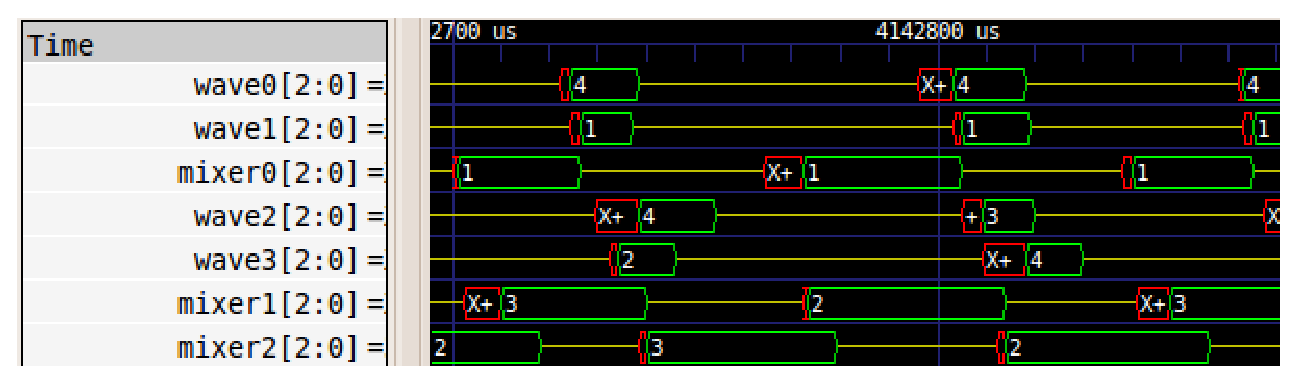
\includegraphics[width=\widefigure]{images/results_xeon/4KB_results_xeon_taskaff.eps}
\caption{\figurecaption{trace of benchmark execution on Xeon with buffer of 4KB using task-affinity}}
\label{fig:4KB_xeon_results_taskaff}
\end{figure}

\begin{figure}[htbp]
\centering
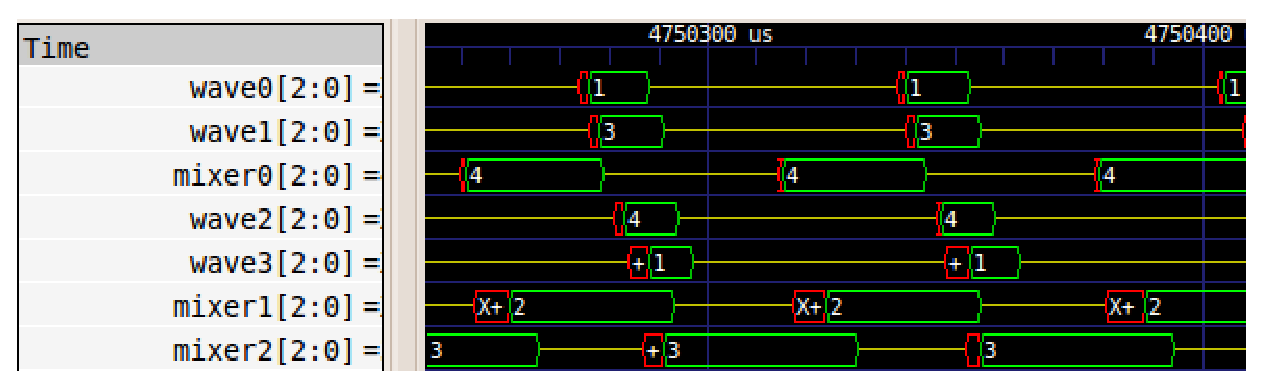
\includegraphics[width=\widefigure]{images/results_xeon/4KB_results_xeon_van.eps}
\caption{\figurecaption{trace of benchmark execution on Xeon with buffer of 4KB using vanilla}}
\label{fig:4KB_xeon_results_van}
\end{figure}

As regard for speedups, we see that, in both Xeon and i7, the estimated average speedups overestimate the real parallelism performed by task-affinity, 
nevertheless they are a good estimate. In fact, for Xeon, we have the estimated average speedup of $2.42$ and the real average speedup of $2.39$: they 
differ by $\sim 1\%$.  While for i7, we have an estimated average speedup of $2.64$ and a real average speedup of $2.5$: they differ by $\sim 5\%$. 
Therefore, we can conclude that scheduling performed by task-affinity can be well approximated by the ideal scheduling, Fig \ref{fig:ideal_scheduling}.

Instead, for vanilla, the estimated average speedups underestimate the real parallelism performed by vanilla. 
In fact, for Xeon, we have an estimated average speedup of $1.86$ and a real average speedup of $2.19$: they differ by $\sim 18\%$. While for i7, we have 
an estimated average speedup of $2.11$ and a real average speedup of $2.26$: they differ by $\sim 7\%$. It is clear from these data, that parallelism
of the scheduling performed by vanilla is greater than parallelism of the ideal scheduling. In fact if we see Fig. \ref{fig:4KB_xeon_results_van} we note 
that there is a fraction of \textit{mixer2} that is executed concurrently with others \textit{waves}, while in ideal scheduling \textit{mixer2} should be 
executed alone.

\item[migrations:] Number of migration is greatly increased. This is not due to architectural details or different buffer dimensions. This fact happens 
because, at each sample, \textit{mixer0} and \textit{mixer1} and \textit{waves} are excuted on the same CPUs. Since in the next sample \textit{waves} are 
waken up during the execution of \textit{mixer0} and \textit{mixer1}, they must be scheduled on CPUs different from which that have executed them in 
the previous sample. For this reason, at each sample, \textit{waves} are executed on different CPUs and, consequently, also other tasks are executed on 
different CPUs at each sample.

\item[cache misses:] Because of worsening of L1 and LLC cache misses, Fig \ref{fig:l1_load_store_xeon} \ref{fig:l2_load_store_xeon}, on Intel Xeon 
predictability of the application is degradated, Fig. \ref{fig:time_avg_var_xeon}, especially using small buffer dimension such as 4KB or 8KB. LLC miss rate 
is greatly increased in task-affinity, because, as explained in the previous chapter, a core can access to data that are in caches of its own die, 
therefore if a task migrates frequently between two different dies, at each migration it will have to warm up LLC cache and cache misses will occur. The 
same goes for L1 cache misses, also in that case a migration between CPUs that are in different dies increase L1 miss rates. Nevertheless with dimension 
greater than 8KB and especially greater than 32KB predictability is improved. On Intel i7, instead, thanks to inclusive shared LLC, a core can access to 
data contained in all caches of other cores, consequently, L1 and LLC cache misses are reduced. The diminishing of cache misses impacts significantly on 
application predictability Fig.\ref{fig:time_avg_var_i7}.

\item[migration functions:] As we can see from Fig. \ref{fig:push_xeon} \ref{fig:push_i7}, in both Xeon and i7, with task-affinity number of call to 
\texttt{push\_rt\_task} is greatly reduced than vanilla. This fact happens because if a CPU is selected according to task-affinity criteria and the enqeued 
task with task-affinity is the next to be executed on selected runqueue, \texttt{push\_rt\_task} for that runqueue is denied. Other tasks on that runqeueue 
that have to migrate will be moved by \texttt{pull\_rt\_task}. Instead, with \textit{pull\_rt\_task} task-affinity is not very effective, in fact, with 
task-affinity, \textit{pull\_rt\_task} it executes more work than in vanilla, Fig. \ref{fig:pull_xeon} \ref{fig:pull_i7}.

\begin{figure}[h]
  \lstset{basicstyle=\footnotesize, language=c, captionpos=b, frame=single,label=lis:steps}
  \lstinputlisting{pull_task.c}
  \label{code:pull_task_code}
  \caption{A portion of the \texttt{pull\_rt\_task} method}
\end{figure}

The explanation is simple: at the line 1559 in Fig. \ref{code:pull_task_code} there is a check for overloading runqueues. If in the system there is any 
overloading runqueue, \textit{pull\_rt\_task} searches which runqueues are overloaded and try to pull task from them. With task-affinity, only 3 
\textit{waves} are executed concurrently and one \textit{wave} has to wait that \textit{mixer2} finish, therefore at each sample there is an overloaded 
runqueue in the system. For this reason, when \textit{pull\_rt\_task} is called, almost certainly it will enter in loop at line 1562 in order to pull tasks 
from overloaded runqueue. With vanilla instead, all waves are executed concurrently, therefore there are less probabilities to have overloaded runqueues. 
It is interesting to note that number of call of \textit{pull\_rt\_task} is equal in both task-affinity and vanilla, because \textit{pull\_rt\_task} 
is called at each context-switch, but obviously, in vanilla \textit{pull\_rt\_tasks} will exit at line 1560. Overhead of \textit{pull\_rt\_task} 
influences predictability of application especially with buffer of 4KB because execution time of each thread is relatively small.

\end{description}

In conclusion, to get a sense of how task-affinity improve performance of benchmark, look at table \ref{tab:final_speedup}, where are reported values of 
metric A2S used to characterize how task-affinity improve throughput and predictability respect vanilla. As we can see, task-affinity is well exploited by
Intel i7, while on Intel Xeon we have some advantage with buffer greater than 4KB.
%%%%%%%%%%%%%%%%%%%%%%%%%%%%%%%%%%%%%%%%%%%%%%%%%%%%%%%%%%%%%%%%%%%%%%%%%%%%%
\section{Intel Xeon}

\begin{figure}[htbp]
\centering
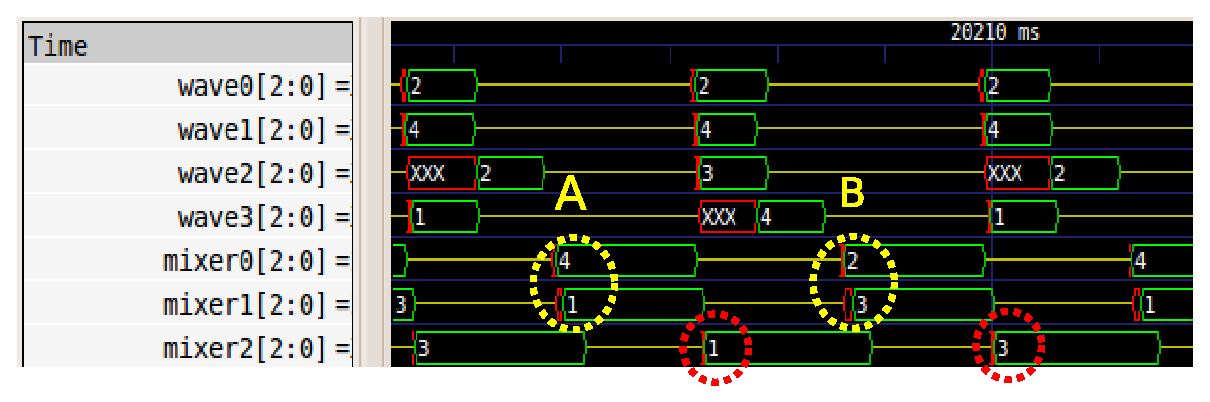
\includegraphics[width=\widefigure]{images/results_xeon/final_xeon.eps}
\caption{\figurecaption{Scheduling performed by task-affinity on Intel Xeon.}}
\label{fig:final_xeon}
\end{figure}

As we can see in Fig. \ref{fig:final_xeon}, the scheduling performed is correct. We see that \textit{mixer2} can precede one of the waves and improve 
parallelism. We see that \textit{mixer0} chooses the best cpu in term of temporal locality, for example: in step A \textit{mixer0} chooses CPU4 and not 
CPU2, because on CPU2 was executed \textit{wave2}, therefore L1 cache could be dirty, instead on CPU4 the last task executed is \textit{wave1}, therefore 
L1 cache should be clean. Also in step B, it is possible to note how \textit{mixer0} take care about the last task executed on CPU4 choosing CPU2.

\begin{table}[tbp]
\centering%
\subfigure[ Average of execution times of each task on serialized execution (Xeon) ]{%
\begin{tabular}{l|c|c|c|c}
	\hline
	& wave & mixer0/1 & mixer2 & serialized exec. time \\ \hline
	$4KB$ & 12.18 & 29.59 & 38.84 & 146.76 \\ \hline
	$8KB$ & 17.74 & 42.72 & 55.57 & 211.98 \\ \hline
	$16KB$ & 31.47 & 70.35 & 88.53 & 355.13 \\ \hline
	$32KB$ & 60.12 & 128.72 & 155.34 & 653.27 \\ \hline
	$64KB$ & 115.42 & 246.2 & 285.62 & 1239.69 \\ \hline
\end{tabular}
\label{tab:task_time_xeon}
}\hspace{4em}
\subfigure[ Portions of serialized execution already expressed in relative terms (Xeon) ]{%
\begin{tabular}{l|c|c|c}
	\hline
	& $P_{0}$ & $P_{1}$ & $P_{2}$ \\\hline
	$4KB$ & 40\%& 33\%& 26\%\\ \hline
	$8KB$ & 39\%& 33\%& 26\%\\ \hline
	$16KB$ & 40\%& 35\%& 25\%\\ \hline
	$32KB$ & 40\%& 37\%& 24\%\\ \hline
	$64KB$ & 40\%& 37\%& 23\%\\ \hline
	$Average$ & 40\%& 35\%& 25\%\\ \hline
\end{tabular}
\label{tab:portion_xeon}
}
\label{tab:time_portion_xeon}
\caption{Times and percentages related to serialized execution of benchmark (Xeon)}
\end{table}

\begin{table}[tbp]
\centering%
\subfigure[ Speedup obtained with task-affinity and with vanilla (Xeon) ]{%
\begin{tabular}{l|c|c|c|c}
	\hline
	& taskaff & vanilla \\ \hline
	$4KB$ & 2.33 & 2.38 \\ \hline
	$8KB$ & 2.34 & 2.22  \\ \hline
	$16KB$ & 2.37 & 2.15 \\ \hline
	$32KB$ & 2.45 & 2.13 \\ \hline
	$64KB$ & 2.47 & 2.09 \\ \hline
	$Average$ & 2.39 & 2.19\\ \hline
\end{tabular}
\label{tab:speedup_xeon}
}\hspace{4em}
\subfigure[ Average of execution time of a sample with task-affinity and vanilla (Xeon) ]{%
\begin{tabular}{l|c|c|c}
	\hline
	& taskaff & vanilla \\ \hline
	$4KB$ & 63.08 & 61.58 \\ \hline
	$8KB$ & 90.6 & 95.54 \\ \hline
	$16KB$ & 150 & 165.23 \\ \hline
	$32KB$ & 266.42 & 306.69 \\ \hline
	$64KB$ & 502.09 & 592.3 \\ \hline
\end{tabular}
\label{tab:final_time_xeon}
}
\label{tab:final_time_speedup_xeon}
\caption{between task-affinity and vanilla on Intel Xeon and Intel i7}
\end{table}


According the showed data it possible to estimate the average speedups for task-affinity and vanilla.

\begin{equation}
  Speedup_{taskaff} = \left( \frac{0.4}{2} + \frac{0.35}{4} + \frac{0.25}{2} \right)^{-1} = 2.42
\label{eq:speedup_xeon_taskaff}
\end{equation}

\begin{equation}
  Speedup_{vanilla} = \left(\frac{0.4}{2} + \frac{0.35}{4} + \frac{0.25}{1} \right)^{-1} = 1.86
\label{eq:speedup_xeon_van}
\end{equation}


\begin{figure}[htbp]
\centering
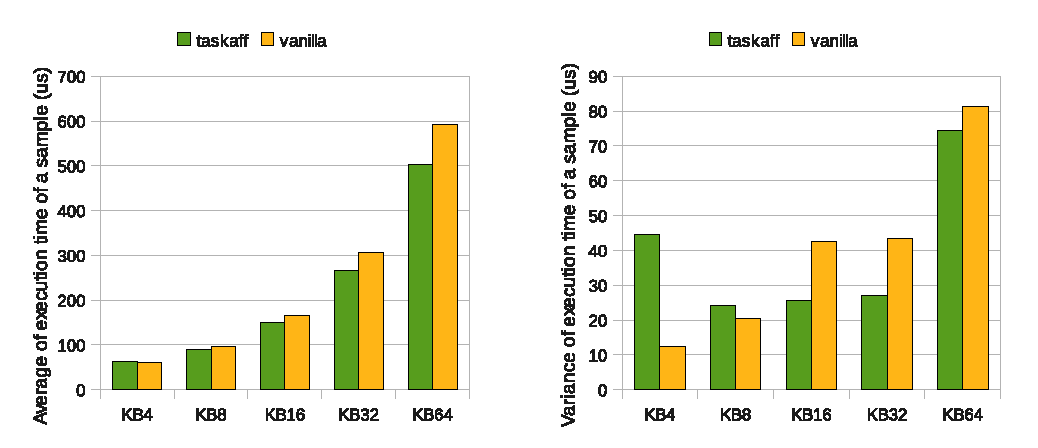
\includegraphics[width=\widefigure]{images/results_xeon/time_avg_var.eps}
\caption{\figurecaption{Average and Variance of execution time of a sample}}
\label{fig:time_avg_var_xeon}
\end{figure}

\begin{figure}[htbp]
\centering
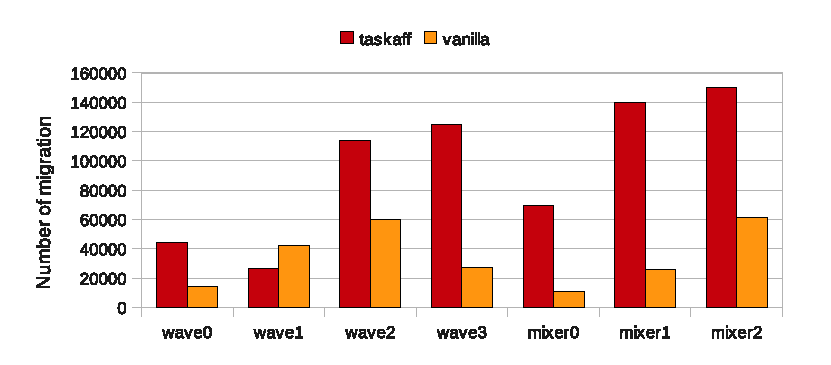
\includegraphics[width=\widefigure]{images/results_xeon/migration_xeon.eps}
\caption{\figurecaption{task migration on Xeon}}
\label{fig:migration_xeon}
\end{figure}

\begin{figure}[htbp]
\centering
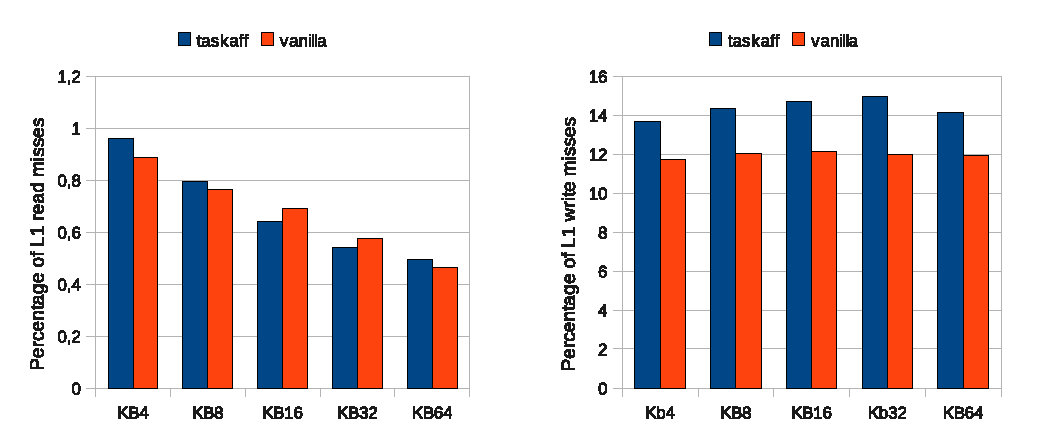
\includegraphics[width=\widefigure]{images/results_xeon/l1_load_store_xeon.eps}
\caption{\figurecaption{L1 Read and Write misses on Xeon}}
\label{fig:l1_load_store_xeon}
\end{figure}

\begin{figure}[htbp]
\centering
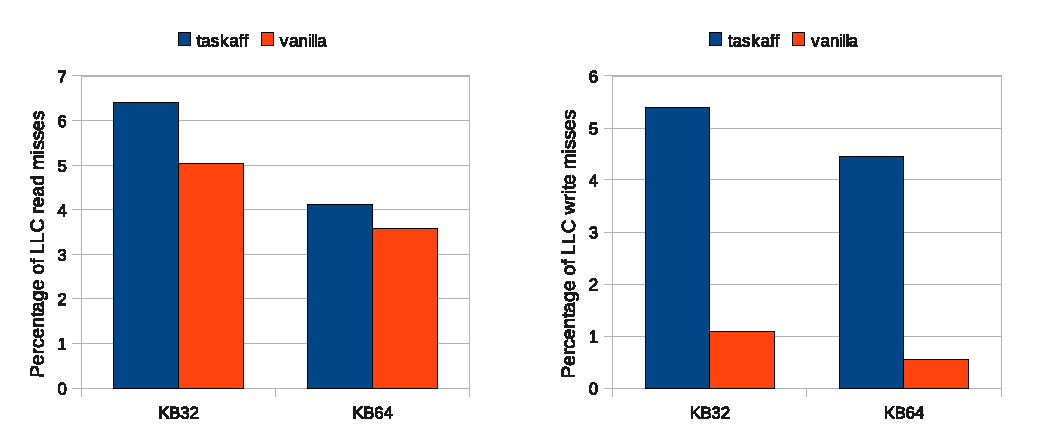
\includegraphics[width=\widefigure]{images/results_xeon/l2_load_store_xeon.eps}
\caption{\figurecaption{LLC Read and Write misses on Xeon}}
\label{fig:l2_load_store_xeon}
\end{figure}

\begin{figure}[htbp]
\centering
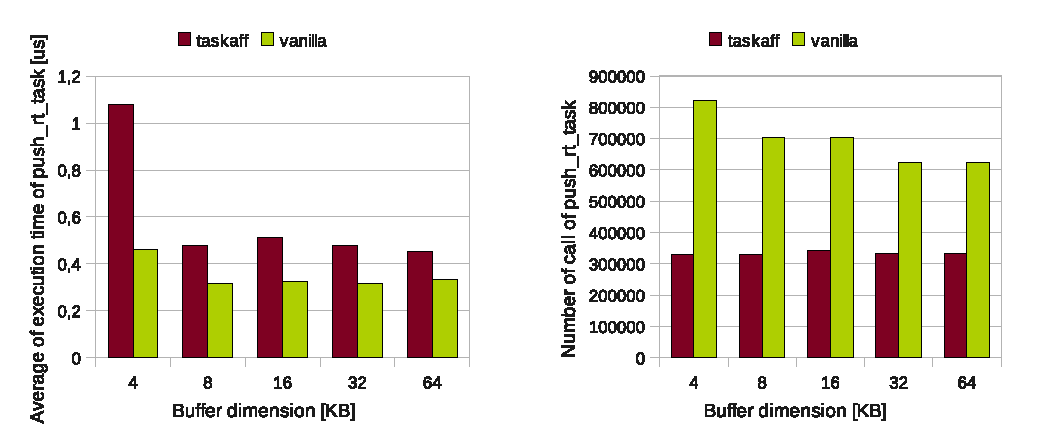
\includegraphics[width=\widefigure]{images/results_xeon/push_xeon.eps}
\caption{\figurecaption{Average of execution time of a call to push\_rt\_task and number of call to push\_rt\_task on Xeon}}
\label{fig:push_xeon}
\end{figure}

\begin{figure}[htbp]
\centering
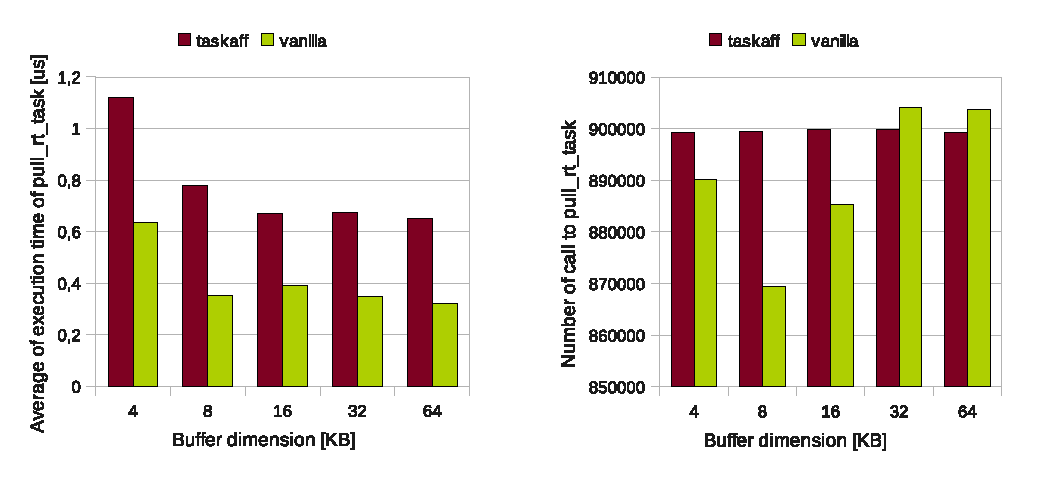
\includegraphics[width=\widefigure]{images/results_xeon/pull_xeon.eps}
\caption{\figurecaption{Average of execution time of a call to pull\_rt\_task and number of call to pull\_rt\_task on Xeon}}
\label{fig:pull_xeon}
\end{figure}

%%%%%%%%%%%%%%%%%%%%%%%%%%%%%%%%%%%%%%%%%%%%%%%%%%%%%%%%%%%%%%%%%%%%%%%%%%%%%
\section{Intel i7}

\begin{figure}[htbp]
\centering
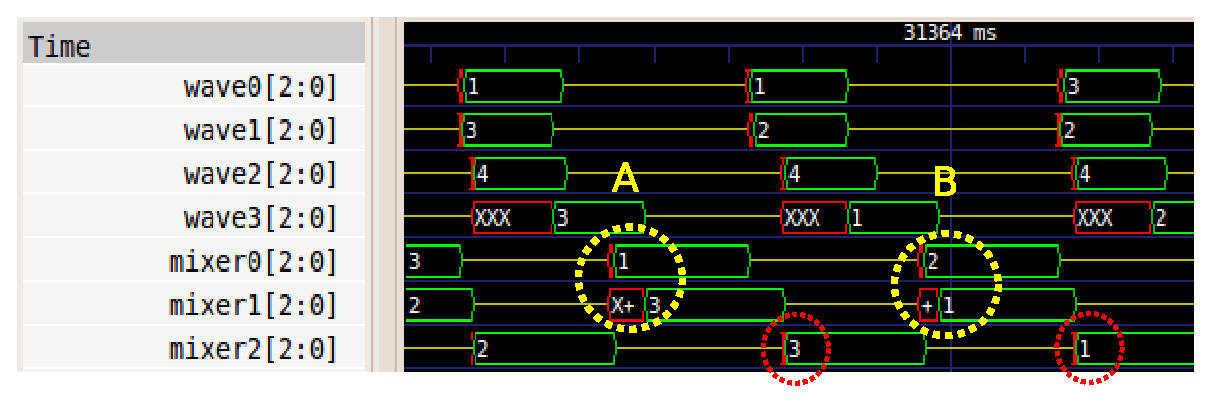
\includegraphics[width=\widefigure]{images/results_i7/final_i7.eps}
\caption{\figurecaption{Scheduling performed by task-affinity.}}
\label{fig:trace_i7}
\end{figure}

We can see from Fig.\ref{fig:trace_i7}, that also in this case the scheduling performed can be approximated with the ideal scheduling, Fig.
\ref{fig:ideal_scheduling}. We can see how in step A and B mixers choose the correct CPUs according to their task-affinity relationships.

Also in this case, according to recorded measurement the estimated average speedups are:

\begin{equation}
  Speedup_{taskaff} = \left(\frac{0.32}{2} + \frac{0.49}{4} + \frac{0.19}{2} \right)^{-1} = 2.64
\label{eq:speedup_i7_taskaff}
\end{equation}

\begin{equation}
  Speedup_{vanilla} = \left(\frac{0.32}{2} + \frac{0.49}{4} + \frac{0.19}{1} \right)^{-1} = 2.11
\label{eq:speedup_i7_van}
\end{equation}

\begin{table}[tbp]
\centering%
\subfigure[execution times of each task on serialized execution (i7) ]{%
\begin{tabular}{l|c|c|c|c}
	\hline
	& wave & mixer0/1 & mixer2 & serialized exec. time \\ \hline
	$4KB$ & 17.86 & 27.31 & 29.25 & 155.31 \\ \hline
	$8KB$ & 33.17 & 46.39 & 51.88 & 277.32 \\ \hline
	$16KB$ & 63.65 & 82.49 & 96.54 & 516.11 \\ \hline
	$32KB$ & 124.85 & 156.46 & 182.3 & 994.59 \\ \hline
	$64KB$ & 250.27 & 279.39 & 356.96 & 1916.82 \\ \hline
\end{tabular}
\label{tab:speedup_xeon}
}\hspace{4em}
\subfigure[ portions of serialized execution already expressed in relative terms (Xeon) ]{%
\begin{tabular}{l|c|c|c}
	\hline
	& $P_{0}$ & $P_{1}$ & $P_{2}$ \\\hline
	$4KB$ & 35\%& 47\%& 18\%\\ \hline
	$8KB$ & 33\%& 48\%& 19\%\\ \hline
	$16KB$ & 32\%& 49\%& 18\%\\ \hline
	$32KB$ & 31\%& 51\%& 19\%\\ \hline
	$64KB$ & 29\%& 52\%& 19\%\\ \hline
	$Average$ & 32\%& 49\%& 19\%\\ \hline
\end{tabular}
\label{tab:speedup_i7}
}
\label{tab:final_speedup}
\caption{Comparison between task-affinity and vanilla on Intel Xeon and Intel i7}
\end{table}

\begin{table}[tbp]
\centering%
\subfigure[ (Xeon) ]{%
\begin{tabular}{l|c|c}
	\hline
	& taskaff & vanilla \\ \hline
	$4KB$ & 2.53 & 2.28 \\ \hline
	$8KB$ & 2.56 & 2.27 \\ \hline
	$16KB$ & 2.51 & 2.18 \\ \hline
	$32KB$ & 2.48 & 2.24 \\ \hline
	$64KB$ & 2.42 & 2.32 \\ \hline
	$Average$ & 2.5 & 2.26\\ \hline
\end{tabular}
\label{tab:speedup_xeon}
}\hspace{4em}
\subfigure[  (Xeon) ]{%
\begin{tabular}{l|c|c}
	\hline
	& taskaff & vanilla \\ \hline
	$4KB$ & 61.44 & 68.25 \\ \hline
	$8KB$ & 108.22 & 122.42 \\ \hline
	$16KB$ & 206.03 & 236.35 \\ \hline
	$32KB$ & 401.53 & 444.38 \\ \hline
	$64KB$ & 793.5 & 826.83 \\ \hline
\end{tabular}
\label{tab:speedup_i7}
}
\label{tab:final_speedup}
\caption{Comparison between task-affinity and vanilla on Intel Xeon and Intel i7}
\end{table}


\begin{figure}[htbp]
\centering
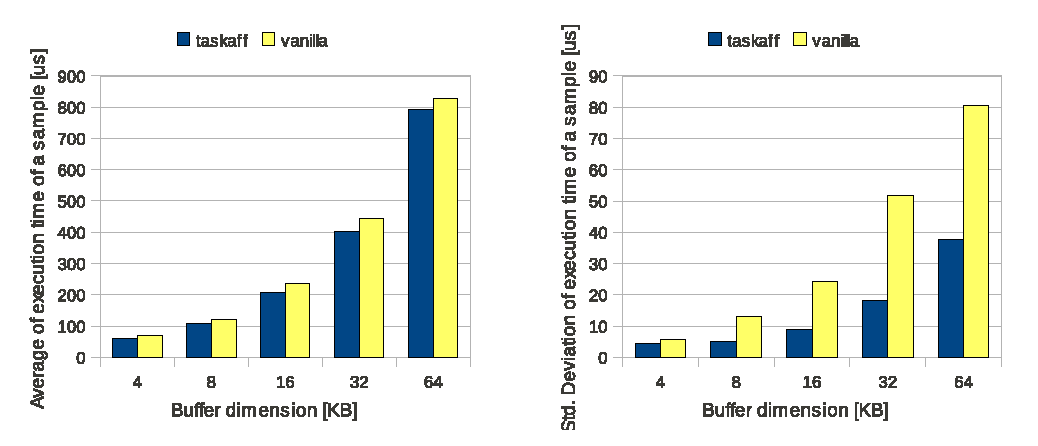
\includegraphics[width=\widefigure]{images/results_i7/time_avg_var_i7.eps}
\caption{\figurecaption{Average and Variance of execution time of a sample}}
\label{fig:time_avg_var_i7}
\end{figure}

%\begin{table}[htbp]
%\begin{center}
%\begin{tabular}{l|c|c|c}
%	\hline
%	& Speedup on i7 \\ \hline
%	& taskaff & vanilla \\ \hline
%\end{tabular}
%\caption{Speedup obtained with task-affinity and with vanilla on i7.}
%\label{tab:speedup_i7}
%\end{center}
%\end{table}

\begin{figure}[htbp]
\centering
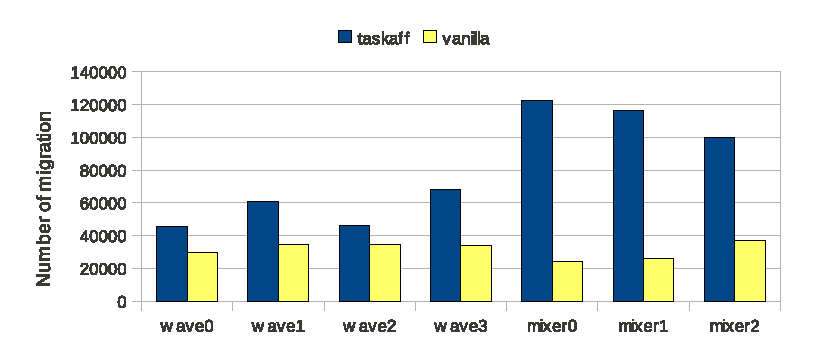
\includegraphics[width=\widefigure]{images/results_i7/migration_i7.eps}
\caption{\figurecaption{task migration on i7}}
\label{fig:migration_i7}
\end{figure}

\begin{figure}[htbp]
\centering
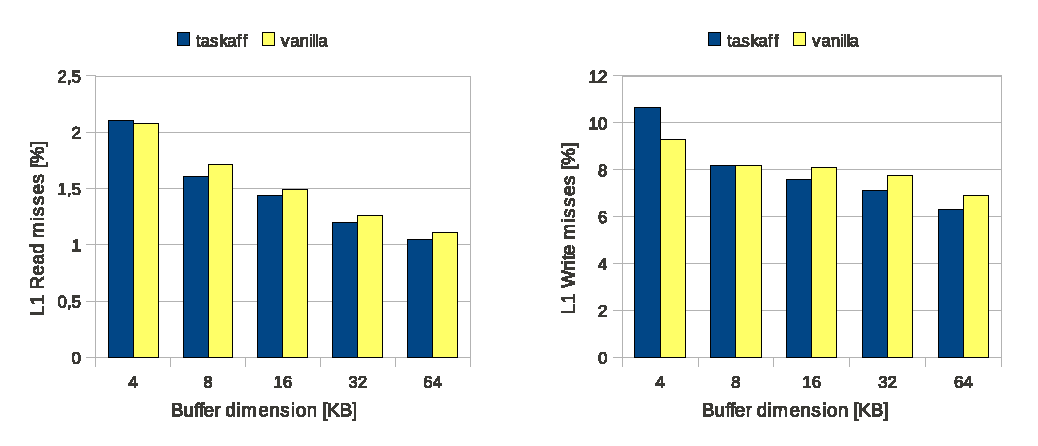
\includegraphics[width=\widefigure]{images/results_i7/l1_load_store_i7.eps}
\caption{\figurecaption{L1 Read and Write misses on i7}}
\label{fig:l1_load_store_i7}
\end{figure}

\begin{figure}[htbp]
\centering
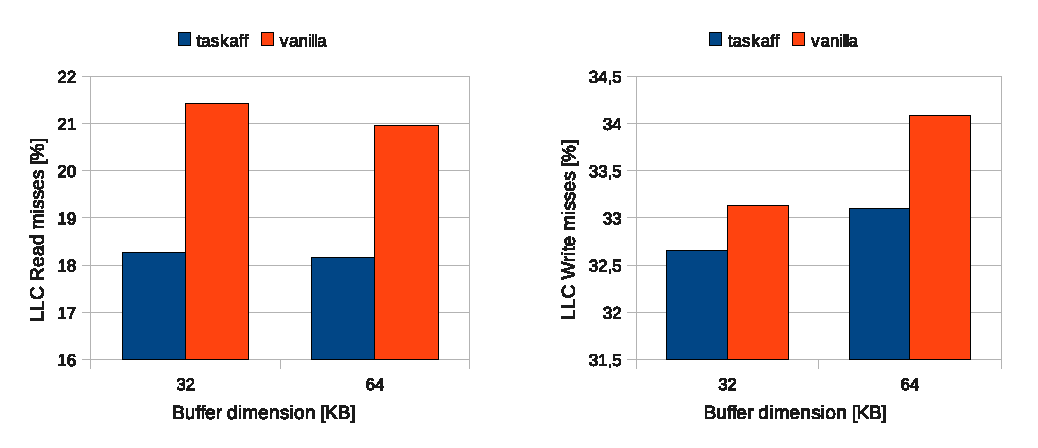
\includegraphics[width=\widefigure]{images/results_i7/l3_load_store_i7.eps}
\caption{\figurecaption{LLC Read and Write misses on i7}}
\label{fig:l2_load_store_i7}
\end{figure}

\begin{figure}[htbp]
\centering
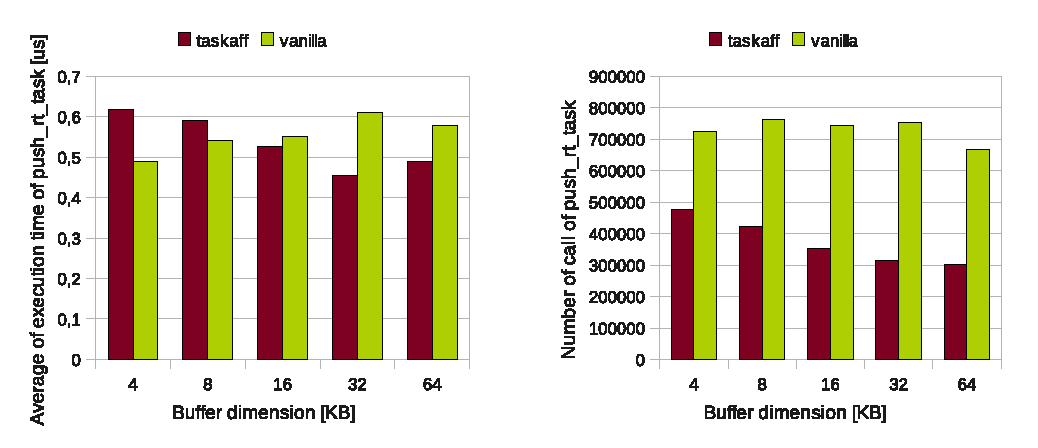
\includegraphics[width=\widefigure]{images/results_i7/push_i7.eps}
\caption{\figurecaption{Average of execution time of a call to push\_rt\_task and number of call to push\_rt\_task on Xeon}}
\label{fig:push_i7}
\end{figure}

\begin{figure}[htbp]
\centering
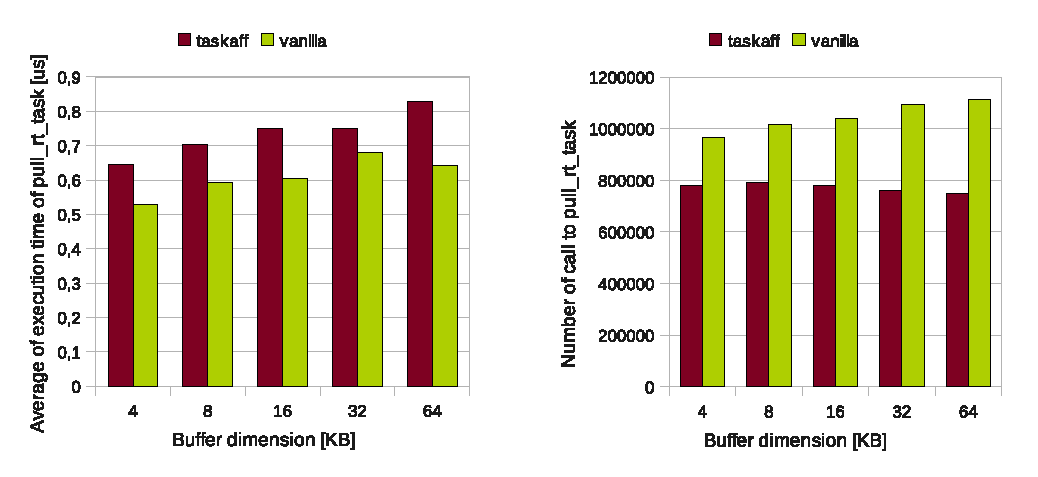
\includegraphics[width=\widefigure]{images/results_i7/pull_i7.eps}
\caption{\figurecaption{Average of execution time of a call to pull\_rt\_task and number of call to pull\_rt\_task on Xeon}}
\label{fig:pull_i7}
\end{figure}

\newpage
%%%%%%%%%%%%%%%%%%%%%%%%%%%%%%%%%%%%%%%%%%%%%%%%%%%%%%%%%%%%%%%%%%%%%%%%%%%%%
\section{AMD Opteron}

\begin{figure}[htbp]
\centering
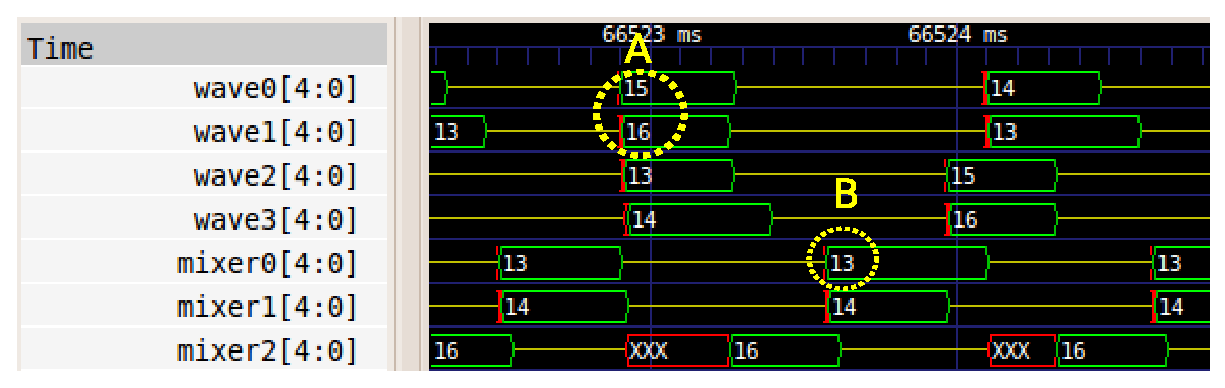
\includegraphics[width=\widefigure]{images/results_AMD/final_AMD.eps}
\caption{\figurecaption{Scheduling performed by task-affinity on AMD Opteron}}
\label{fig:trace_AMD}
\end{figure}

\begin{figure}[htbp]
\centering
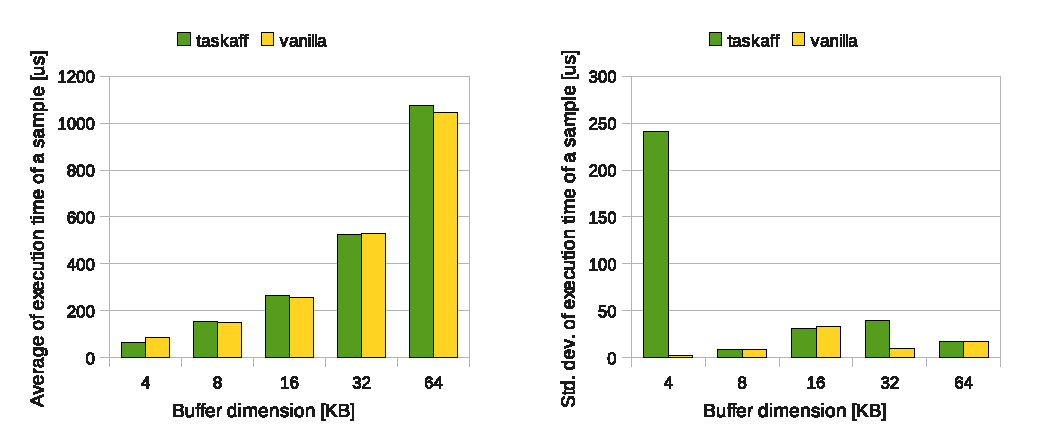
\includegraphics[width=\widefigure]{images/results_AMD/time_avg_var_AMD.eps}
\caption{\figurecaption{Average and Variance of execution time of a sample}}
\label{fig:time_avg_var_AMD}
\end{figure}

Task-affinity on this machine doesn't work. We can see in step B that \textit{mixer0} doesn't choose the correct CPU. The incorrect behaviour of 
task-affinity is also reflected by Fig. \ref{fig:time_avg_var_AMD}, where we can see a worsening of throughput and predictability. We have executed 
task-affinity on this machine in order to investigate which is task-affinity behaviour on NUMA architectures. According these results, we conclude that 
it is necessary a revision of task-affinity in order to use it also on NUMA architectures.

TODO correggi i numeri
\begin{table}[tbp]
\centering%
\subfigure[ Value of A2S on Xeon ]{%
\begin{tabular}{l|c|c|c}
	\hline
	& taskaff & vanilla & speedups \\ \hline
	$4KB$ & 76,45 & 68,63 & -- \\ \hline
	$8KB$ & 100,43 & 104,55 & 4\%\\ \hline
	$16KB$ & 160,15 & 178,27 & 10\%\\ \hline
	$32KB$  & 276,84 & 319,85 & 13\%\\ \hline
	$64KB$  & 519,35 & 610,35 & 17\%\\ \hline
\end{tabular}
\label{tab:speedup_xeon}
}\hspace{4em}
\subfigure[ Values of A2S on i7 ]{%
\begin{tabular}{l|c|c|c}
	\hline
	& taskaff & vanilla & speedups \\ \hline
	$4KB$ & 70,47 & 79,91 & 12\%\\ \hline
	$8KB$ & 118,32 & 148,34 & 20\%\\ \hline
	$16KB$ & 223,61 & 284,8 & 21\%\\ \hline
	$32KB$  & 437,76 & 548,08 & 20\%\\ \hline
	$64KB$  & 868,97 & 987,7 & 12\%\\ \hline
\end{tabular}
\label{tab:speedup_i7}
}
\label{tab:final_speedup}
\caption{Comparison between task-affinity and vanilla on Intel Xeon and Intel i7}
\end{table}

